% Modelo de Dissertação em Latex para o PPG em Engenharia Elétrica - Sistemas Eletrônicos da UERJ
% Este modelo foi adaptado da versão disponibilizada no site da Engenharia Elétrica da UERJ
% http://www.pel.uerj.br/publico/Modelo_LaTeX_Dissertacao_UERJ.rar
% http://www.pel.uerj.br/defesas/
%
% 
%
% 
%
% 
% Atualizações:
% Felipe M. - 20/06/2012
% Fernando Lima - 15/07/2015
%





\documentclass[a4paper,12pt,oneside,openany]{uerj}

\usepackage[english,brazil]{babel}
%\usepackage[latin1]{inputenc}
\usepackage[utf8]{inputenc}
\usepackage{enumerate}
\usepackage{cite}
\usepackage{epsf,epsfig,./packages/psfig}
\usepackage{./packages/pagina}
\usepackage{indentfirst}
\usepackage{theorem}
\usepackage{fancyhdr}
\usepackage{setspace}
\usepackage{boxedminipage}
\usepackage{float}
\usepackage{makeidx}
\usepackage{amsmath}
\usepackage[hidelinks]{hyperref}




%%%%%% Definições %%%%%%%
\newtheorem{deff}{Definição}[section]
\numberwithin{equation}{chapter}

\theoremstyle{plain}

\bibliographystyle{./bib/abnt-num}



%%%%% DOC %%%%%%%%%%%%


\makeindex


\begin{document}


%%% Modifique aqui seu Nome, título do trabalho e data

\newcommand{\setNomeAluno}{Fernando de Oliveira Lima}
\newcommand{\setTitulo}{Sistema Escalável para Aplicações de Internet das Coisas utilizando MQTT}
\newcommand{\setLocationDate}{Rio de Janeiro\\2018} % Coloque aqui a localização e data
\newcommand{\setApprovalDate}{28 de Agosto 2018}


\hypersetup{
    colorlinks,
    citecolor=black,
    filecolor=black,
    linkcolor=black,
    urlcolor=black,
    linktoc=all
}

\thispagestyle{empty}\begin{titlepage}
\begin{center}

	\vspace{-0.5cm}

  \begin{figure}[hbt!]
		\begin{flushleft}
		   
\includegraphics[width=3.44cm,height=3.17cm]{./01_Pre_textuais/figures/logo_uerj_pb.png}
		\end{flushleft}
	\end{figure}
	\vspace{-4cm}

  \hspace{2cm}\large{\textbf{Universidade do Estado do Rio de Janeiro}}\\
  \hspace{2cm}\large{Centro de Tecnologia e Ciências}\\
  \hspace{2cm}\large{Faculdade de Engenharia}\\

  \hspace{2cm}\large{}\\
  \hspace{2cm}\large{}\\
  \hspace{2cm}\large{}\\
  \hspace{2cm}\large{}\\

  \par
  \large{\setNomeAluno}

  \hspace{2cm}\large{}\\
  \hspace{2cm}\large{}\\
  \hspace{2cm}\large{}\\
  \hspace{2cm}\large{}\\


  \par
  \large\textbf{\setTitulo}


  \par\vfill
  \setLocationDate

\end{center}
\end{titlepage}
\pagebreak\thispagestyle{empty}\begin{center}

\setNomeAluno
% \vfill
\vspace{2cm}

\textbf{\setTitulo}

\vspace{1.0cm}

\begin{figure}[hbt!]
\begin{center}

\includegraphics[width=10.48cm,height=10.8cm]{./01_Pre_textuais/figures/logo_uerj_gnd_pb.png}
\end{center}
\end{figure}

\vspace{-9cm}
\begin{flushright}
\parbox{8cm}{
\singlespacing{Projeto de Graduação apresentado, como requisito parcial para obtenção do grau de Engenheiro Eletricista, á Faculdade de Engenharia, da Universidade do Estado do Rio de Janeiro. Ênfase: Sistemas Eletrônicos.}
}
\end{flushright}

\vspace{4.0cm}


\begin{table}[h!]
\centering
\begin{tabular}{ll}
Orientadores: & Prof. Michel Tcheou, DSc\\
					& Prof. Lisandro Lovisolo, DSc\\
\end{tabular}
\end{table}


\par\vfill
%\vspace{2cm}

\setLocationDate
\end{center}
\pagebreak\thispagestyle{empty}% Depois de preparar seu trabalho, você deverá enviá-lo para a Biblioteca CTC/B para avaliação do formato e elaboração da Ficha catalográfica.
% Com a ficha pronta (fornecida pela Biblioteca), você poderá alterar este trecho do trabalho em definitivo.
%
% Para este processo, enviei a dissertação em PDF para o email: ctcb.uerj.bdtd@gmail.com (Tratei de todos os detlahes com a Sra. Márcia)
% Qualquer dúvida, veja os contatos da Biblioteca no site da Rede Sirius: http://www.rsirius.uerj.br/
% 


\begin{titlepage}
	\begin{center}
\vfill
\singlespacing
	\vspace*{95mm}
	{CATALOGAÇÃO NA FONTE\\ \vspace{1.5mm}
	UERJ\,/\,REDE SIRIUS\,/\,BIBLIOTECA CTC/B}\\
	\vspace{1.5mm}
	\begin{boxedminipage}{140mm}
	\begin{minipage}{5mm}
		\vspace{-84mm}
		S237
	\end{minipage}
	\hfill
	\raisebox{8.5mm}{
	\begin{minipage}[top]{115mm}
		\vspace*{5mm}

		de Oliveira Lima, Fernando\\
		\phantom{XX}\setTitulo\,/\,\setNomeAluno -- 2018.\\
		\phantom{XX}\pageref{LastPage}\,f.\\
		\phantom{XX}\\
		\phantom{XX}Orientadores: Michel Pompeu Tcheou, Lisandro Lovisolo.\\
       		\phantom{XX}Projeto de Graduação -- Universidade do Estado do Rio de Janeiro, Faculdade de Engenharia.\\
		\phantom{XX} Bibliografia: p.43\\
		\phantom{XX} \\
		\phantom{XX} Texto a ser informado pela biblioteca
	\end{minipage}}
	\vspace*{5mm}
	\begin{flushright}
	 CDU~621:528.8
	\end{flushright}
    \vspace{1mm}
	\end{boxedminipage}\\
	\end{center}
%
	Autorizo, apenas para fins acadêmicos e científicos, a reprodução total ou parcial desta dissertação, desde que citada a fonte.\\
	\noindent
	\begin{tabular}{ccc}
	\phantom{XXXXXXXXXXXXXXXXXXXXXXXXXXXXXX}&	 \phantom{XX}	&	\phantom{XXXXXXXXXXXXXXXX}	\\
	\phantom{XXXXXXXXXXXXXXXXXXXXXXXXXXXXXX}&	 \phantom{XX}	&	\phantom{XXXXXXXXXXXXXXXX}	\\
	\cline{1-1}\cline{3-3}
	Assinatura &		&	Data
	\end{tabular}
\end{titlepage} 
\pagebreak\thispagestyle{empty}\addtocounter{page}{+1}
\begin{center}

\setNomeAluno

\vspace{1cm}

\textbf{\setTitulo}

\end{center}

\vspace{.4cm}

\begin{flushright}
\parbox{8cm}{
\singlespacing{Trabalho de Conclusão de Curso apresentado, como requisito parcial para obtenção do título de Bacharel em Engenharia Elétrica ênfase em Sistemas Eletrônico, da Universidade do Estado do Rio de Janeiro.}
}
\end{flushright}

\vspace{.6cm}


% insira abaixo a data de sua defesa
% Caso não tenha defendido ainda, deixe em branco

\noindent Aprovado em: \setApprovalDate

\noindent Banca Examinadora:


%
%
% Os professores da UERJ DEVEM ser citados primeiro, independente de quem seja o orientador.
%
%



\vspace{.7cm}

\begin{flushright}
\parbox{12cm}{

\singlespacing

\hrulefill \\

\vspace{-.4cm}
Prof. Dr. Michel Pompeu Tcheou (Orientador)
\newline
Departamento de Eletrônica e Telecomunicações  da UERJ
\vspace{.7cm}

\hrulefill \\

\vspace{-.4cm}
Prof. Dr. Lisandro Lovisolo (Orientador)
\newline
Departamento de Eletrônica e Telecomunicações  da UERJ
\vspace{.7cm}


\hrulefill \\

\vspace{-.4cm}
Prof. Dr. Nome do Professor 3
\newline
Universidade Federal do Rio de Janeiro - UFRJ - COPPE
\vspace{.7cm}

\hrulefill \\

\vspace{-.4cm}
Prof. Dr. Nome do Professor 4
\newline
Instituto de Geociências da UFF
\vspace{.7cm}
}
\end{flushright}
\vfill

\begin{center}
\setLocationDate
\end{center}

\pagebreak\thispagestyle{empty}\begin{center}
\textbf{DEDICATÓRIA}
\end{center}

$\!$\\

%\vspace{1cm}

Aqui entra sua dedicatória.




\pagebreak\thispagestyle{empty}\begin{center}
\textbf{AGRADECIMENTO}
\end{center}

$\!$\\

Agradeço aos amigos e aos não tão amigos, que igualmente fizeram parte da minha evolução como ser humano e cidadão. Todas as pessoas que passaram na minha vida contribuíram um pouco para esse momento, não há como saber onde todas estão, mas se um dia lerem esse texto, quero que saiba que eu agradeço a companhia e o aprendizado.

Não poderia ficar de fora, é claro, todos aqueles que de Alguma forma foram meus mentores. Meus professores ao longo da vida, em especial os dois orientadores desse projeto, já os conheço a quase sete anos, fizeram parte da minha formação, me deram oportunidades e ajudaram a concretizar esse trabalho. Agradeço de coração, que mais oportunidades de nos encontrar surjam, e desejo todo o sucesso possível e uma vida feliz e confortável.

Fica meu agradecimento aqui também para essa instituição linda e maravilhosa, que não é fácil de lidar, muitas vezes pareceu que ia nos abandonar, mas trouxemos ela de volta, cada um com sua parte. Obrigado UERJ, por uma parte inesquecível da minha vida e por todas as pessoas que conheci dentro deste universidade.

E se você estiver lendo esse texto, sim, você mesmo leitor! Agradeço seu prestígio, mesmo se você tiver ignorado completamente esta parte. Espero que tenha aprendido um pouco. O texto é para Ciência, para a Tecnologia e para você.

 
%\pagebreak\thispagestyle{empty}\input{./01_Pre_textuais/Epigrafe}    % não coloquei epígrafe no meu trabalho, mas fica aqui a chamada comentada.
\pagebreak\thispagestyle{empty}\begin{center}
\textbf{RESUMO}
\end{center}

%
% O resumo deve ser organizado em apenas um parágrafo mesmo.
% O número de folha é o número de páginas do PDF -2. Isto ocorre pois na versão final (capa dura) a capa é removida e as duas primeiras páginas são impressas em uma % folha apenas (frente e verso).
%

$\!$\\

\hspace{-1.3cm}\textbf{LIMA}, Fernando \textit{\setTitulo}. 105 f. Trabalho de Conclusão de Curso~(Engenharia Elétrica ênfase em Sistemas Eletrônicos) - Faculdade de Engenharia, Universidade do Estado do Rio de Janeiro (UERJ), Rio de Janeiro, 2018.

\vspace{.2cm}

No meio da revolução dos dados, cresce o interesse em sistemas de comunicação entre máquinas e sistemas de compartilhamento e visualização de dados  sobre dispositivos, seja numa fábrica ou em residências. Este trabalho apresenta um sistema para aplicações de internet das coisas(IoT) utilizando MQTT, um protocolo de aplicação para comunicação entre dispositivos que enviam dados telemétricos. É  a \textit{língua franca} para publicação de dados telemétricos via TCP/IP, com persistência de dados em banco MongoDB. O sistema englobará todos os setores de aquisição dos dados a camada de aplicação em consoles, com o objetivo de facilitar a implementação de aplicações eficientes em cada cenário.

\vspace{1cm}

\hspace{-1.3cm}Keywords: IoT, MQTT, industry .
\pagebreak\thispagestyle{empty}\begin{center}
\textbf{ABSTRACT}
\end{center}

$\!$\\

% O resumo em inglês deve ser organizado em apenas um parágrafo mesmo.

In the verge of the data revolution, a growing interest in communication sytems between machines and the sharing systems of telemetric data on devices rises, whether in a factory or in a residence. This work presents a system for Internet applications of things (IoT) using MQTT, an application protocol for communication between devices that shares telemetri data . It is the \textit{língua franca} for publishing telemetric data via TCP / IP, with data persistion using MongoDB. The system will  encompass all sectors of data acquisition to the application layer in consoles, facilitating implementations of applications in each scenario.

\vspace{1cm}

\hspace{-1.3cm}Keywords: IoT, MQTT, industry .

\fancypagestyle{plain}{
\fancyhf{} % clear all header and footer fields
\renewcommand{\headrulewidth}{0pt}
\renewcommand{\footrulewidth}{0pt}}
\pagestyle{plain}

\pagebreak

\def\listfigurename{LISTA DE FIGURAS}\listoffigures
\def\listtablename{LISTA DE TABELAS}\listoftables
%\newpage

\begin{center}
\textbf{LISTA DE SIGLAS}
\end{center}
$\!$\\

\begin{tabular}{lll}
IoT & \hspace{1cm} & Internet das Coisas \\
NB &\hspace{1cm} &  Narrow Band Networks \\
A/D & \hspace{1cm} & Analógico-Digital \\
DB &  \hspace{1cm} & Banco de Dados \\
IaaS & \hspace{1cm} & Infrastructure as a Service \\
MCU & \hspace{1cm} & Micro-Controller Unit \\
\end{tabular}
    % não coloquei LISTA DE SIGLAS no meu trabalho, mas fica aqui a chamada comentada.
\def\contentsname{SUMÁRIO}\tableofcontents

\fancypagestyle{plain}{
\fancyhf{} % clear all header and footer fields
\fancyhead[R]{\thepage}
\setlength{\voffset}{-1cm}
\setlength{\headsep}{1cm}
\renewcommand{\headrulewidth}{0pt}
\renewcommand{\footrulewidth}{0pt}}

\pagestyle{plain}

\pagebreak
\addcontentsline{toc}{chapter}{\hspace{1.7cm}\bfseries INTRODUÇÃO}
\noindent\textbf{INTRODUÇÃO}
$\!$\\

O cenário atual do desenvolvimento tecnológico encontra-se no meio de uma quarta revolução industrial. Nunca se produziu tantos dados e utilizou-se redes como a própria internet para propaga-los. É de se esperar que tanto o cenário acadêmico e o próprio mercado demandem inovações para o compartilhamento desses dados em tempo real ou próximo disso. Fazendo aquecer o mercado que engloba transporte, análise e inteligência de dados.

Essa revolução possui um nome, Indústria 4.0. Ela engloba todas as áreas que lidam com dados, da análise à rede que distribui os dados. E dentre estas áreas complexas, que envolvem quase todos os subgrupos da engenharia elétrica, encontra-se a Internet das Coisas, ou IoT, como iremos nos referenciar nesta dissertação.

A Internet das Coisas é a rede ou sistema que adquire, compartilha e aplica dados de dispositivos previamente equipados para medir e divulga-los. Ela é derivada métodos de comunicação entre máquinas e telemetria. Pode ser dissecada em três camadas de aquisição, comunicação e aplicação destes dados e pode ser implementada utilizando diversos protocolos de comunicação, dependendo da tecnologia disponível. É importante que o sistemas IoT deva ser construído de forma a atender a aplicação de uma forma eficiente, porém tal tarefa não é fácil nem simples.

Este projeto propõe uma interface que fornece comunicação entre as diferentes tecnologias e camadas de rede, de forma que o usuário só se preocupe em  implementar e configurar a interface para mapear a melhor opção de ferramentas para a aplicação. O projeto lida com protocolos baseados na pilha TCP/IP, uma unanimidade em redes que se comunicam com a internet. Podendo se estender para outras protocolos de aplicações de escopo fechado. O foco está no protocolo de aplicação MQTT (Message Queuing Telemetry Transport), um protocolo que trabalho em cima do TCP/IP, leve e extremamente utilizado para compartilhamento dados telemétricos, de estado e de pequenas mensagens. Oferecendo uma API para tanto a aquisição assim como o recebimento e armazenamento destes dados.

 



\chapter{Indústria 4.0 e Internet das Coisas}
\label{chapter:industria_4_0_iot}

A revolução dos dados atingiu praticamente todas as áreas de engenharia elétrica, desde a eletrônica, desenvolvendo dispositivos capazes de receber dados telemétricos, processa-los e envia-los para demais hubs, a servidores de armazenamento de dados, recorrentemente chamados de Data Warehouses. Esse conjunto de mudanças engloba a Indústria 4.0, uma indústria que capta dados de suas máquinas em tempo real em larga escala, analisa, armazena, e utiliza inteligência artificial e estatística, para tomada de decisões estratégicas, contando sempre , é claro, com ajustes humanos.

\section{Internet das Coisas}
\label{section:iot}

"A Internet das Coisas tem o potencial de mudar o mundo. Assim como a Internet fez. Talvez até mais"\cite{ashton:iot}. Uma tradução livre de Rampim \cite{Rampim:iot} da frase de Kevin Ashton, cofundandor do Auto-ID Center, em 1999. Apesar de ser um nome feito somente para chamar atenção, foi a primeira citação da expressão Internet das Coisas, e de lá vingou.

Dentre o meio da Indústria 4.0, encontra-se a internet das coisas ou IoT, responsável por estruturar as aplicações de aquisição, transmissão e armazenamento de dados a serem analisados. Não é uma surpresa que este setor envolva áreas como eletrônica, computação e telecomunicações em um pacote só. De fato suas camadas são mundos diferentes interligados a um propósito : transmitir dados sobre um dispositivo e/ou para um dispositivo em tempo real. Segundo a Cisco IBSG \cite{cisco:ibsg}, há mais objetos conectados que a própria população mundial, fazendo com que o ano de 2009 ser considerado o ano de nascimento do IoT.

Pode-se definir IoT como a estrutura que comunica dispositivos em rede, permitindo a transmissão de dados sobre estes em tempo real. É a ponte que permite a troca de informações sobre um dispositivo, qual seu status, seu desempenho, suas condições físicas e do ambiente ao seu redor. Mas, para que este ciclo esteja completo é necessário camadas que desempenham tarefas específicas, para que o dado chegue a quem ou a o que está esperando.

\section{As Camadas do IoT}
\label{section:camadas_iot}

Semelhante as camadas de rede, as camadas de IoT também exercem funções específicas no transporte de dados, e a camada acima não necessariamente precisa saber como a inferior funciona, somente precisa dos dados que esta camada entrega e executar suas tarefas sobre estes até chegar ao destino especificado.

\begin{figure}[h!]
\label{fig:1.1.0/camadas_iot}
\centering
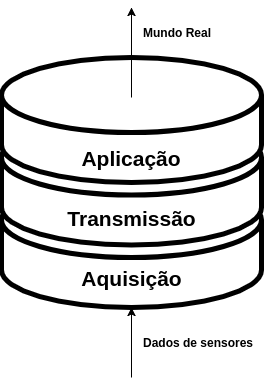
\includegraphics[width=5cm]{./02_Capitulos/02_Cap1/figures/iot_stack}
\caption{As três camadas do IoT, dos sensores ao mundo real}
\end{figure}

A primeira camada é a de aquisição de dados, que lida com o mundo físico e amostra estes dados através de sensores e conversores A/D, também realiza o processamento para entregar em um formato adequado para transmissão e entendível do outro lado, dependo da aplicação. A segunda camada é a camada de transmissão, onde estão, efetivamente, as camadas de rede embutidas. Como o nome já denuncia, ela lida com os aspectos de rede e comunicação para que o dados cheguem as seus destinos. E por último temos a camada de aplicação, a mais abrangente e que envolve maior poder computacional. Ela recebe os dados e lida com os processos de aplicação destes dados, seja análise, visualização, armazenamento ou a estruturação destes.

\subsection{Aquisição}
\label{subsection:aquisicao}

A etapa de aquisição está inserida diretamente no contexto de dados físicos, geralmente são hardwares menos complexos, focados em processamento de dados e entrada e saída com conversão analógico-digital. Se comunicam com sensores ou centrais de controle lógico. São responsáveis por:

\begin{itemize}
	\item Receber dados de sensores;
	\item conversão A/D;
	\item Processamento e calibragem de valores;
	\item Envio de dados em tempo real;
\end{itemize} 

Para atender essas tarefas, não é necessário grande poder de processamento, microcontroladores ou microprocessadores são capazes de atender tais necessidades se acompanhados de módulos de rede e portas I/O, assim como a implementação do software. Veremos dois exemplos no capítulo de implementação do projeto, que utilizam tanto MCU (Micro-Controller Units) ou Consoles com Sistemas Operacionais leves.
 

\subsection{Transmissão}
\label{subsection:transmicao}

Esta camada é o coração do IoT. A forma de transmissão define quais dispositivos eletrônicos e qual sua especificação técnica necessária para os quesitos de transmissão. Também define como os softwares da camada de aplicação e aquisição devem ser implementados baseado na estrutura da pilha de rede que será usada para transmitir.

Na próxima seção, veremos sobre a camada de rede e suas diversas formas de implementação. É importante que esta camada seja definida da melhor forma a atender sua aplicação, atendendo aspectos: 
\begin{itemize}
\item quantidade de dados transmitido;
\item número de acessos; 
\item distância entre dispositivos;
\item segurança;
\end{itemize}

\subsection{Aplicação}
\label{subsection:aplicacao}

A camada de aplicação encabeça a pilha do IoT. É ela que de fato trata os dados e realiza as aplicações deste. Ela disponibiliza os dados para o mundo real, podendo exercer múltiplas funções simultâneas incluindo:

\begin{itemize}
\item Armazenamento e Análise;
\item Visualização; 
\item Inteligência e aprendizado;
\item Serviços e servidores;
\item Gerenciamento e configuração;
\end{itemize}

Nesta camada estão presentes os endpoints apontados pela camada de aquisiçao, o destino dos dados. Bem assim como os servidores que gerenciam os clientes (geralmente implementados na camada de aquisição) e serviços e configurações oferecidos pelo sistema em si.

\section{Camadas de Rede}
\label{section:camadas_de_rede}

Como visto anteriormente, a camada de transmissão basicamente define a infraestrutura do sistema. Ela é construído com as camadas de rede como base. Portanto definir as camadas de rede e seus protocolos é definir a camada de transmissão em si.

Redes de computadores são complexas com diferentes aspectos a se preocupar. Dividir em camadas permite modularizar a implementação da rede, de modo que cada camada tenha uma tarefa na estrutura de comunicação dos aspectos físicos ao software. Como a camada de cima não precisa saber sobre os detalhes e especificações da camada de baixo, as mudanças de uma parte do sistema é transparente para o resto do sistema. Existem diversas formas de implementação de camadas, mas todas se baseiam em um modelo de referência, o modelo OSI \cite{Zimmermann:1988:ORM:59309.59310}.


\begin{figure}[h!]
\label{fig:1.2.0/modelo_osi_tcpip}
\centering
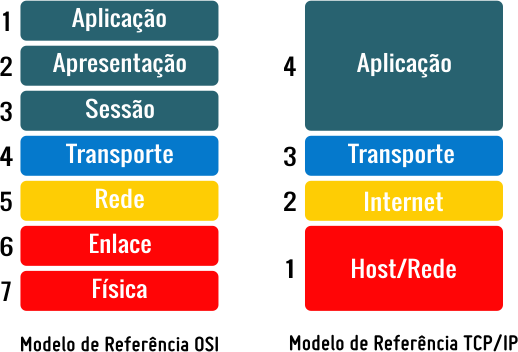
\includegraphics[width=8cm]{./02_Capitulos/02_Cap1/figures/modelo_osi_tcpip}
\caption{Diferenças entre OSI e TCP/IP em suas camadas}
\end{figure}

Baseado no modelo OSI. Temos o modelo TCP/IP \cite{TCPIP}, utilizado na internet e base para protocolos de aplicação muito utilizados como HTTP, WebSocket e MQTT. Em ambos cada camada exerce uma tarefa com seu respectivo protocolo, como resumido na tabela \ref{table:1.2.0}.

\begin{table}[h]
\centering
\caption{As camadas e e suas funções}
\begin{tabular}{|l|l|}
\hline
\multicolumn{1}{|c|}{CAMADA} & \multicolumn{1}{c|}{DETALHES}                                                  \\ \hline
7 - Aplicação                & Define instruções específicas da aplicação          						    \\ \hline
6 - Apresentação             & Formatação dos dados, conversão dos dados                     					\\ \hline
5 - Sessão                   & Negociação e conexão com outros nós, analogia                                \\ \hline
4 - Transporte               & Oferece métodos para a entrega de end-to-end                        			\\ \hline
3 - Rede                     & Roteamento de pacotes em uma ou várias redes                                 \\ \hline
2 - Enlace                   & Detecção de erros;                                                            \\ \hline
1 - Física                   & Aspectos físicos da transmissão \\ \hline
\end{tabular}
\label{table:1.2.0}
\end{table}


O foco desta literatura está na camada de aplicação e suas funcionalidades. Apesar de diferentes tecnologias utilizarem diferentes camadas abaixo, serão especificas características de protocolos construídos em cima do TCP/IP, por seu uso na Internet e redes industriais, e que sejam eficientes em trocas de mensagens em tempo real.



% inserir demais capítulos aqui
% -----------------------------
% -----------------------------
% -----------------------------
% -----------------------------





\pagebreak
\addcontentsline{toc}{chapter}{\hspace{1.7cm}\bfseries CONCLUSÃO}
\noindent\textbf{CONCLUSÃO}
$\!$\\


% Falar sobre o projeto em si
Nesta dissertação, foram apresentados todos os aspectos de hardware, software e econômicos em seus capítulos. Cada um explicando o planejamento a a forma de implementação da ideia, de modo a deixar claro ao leitor como construir e utilizar o sistema como um todo.

O sistema segue sua proposta de escopo aberto, escalável e de baixo custo. Foram apresentadas plataformas de hardware aberto, oferecendo a possibilidade de uma organização ou empresa distribuírem suas próprias versões e baratear ainda mais os custos em larga escala. Os softwares são de escopo aberto e licenças altamente permissíveis, o que significa que possuem versões gratuitas e escaláveis, de modo a também oferecerem a possibilidade de criar versões personalizadas.

A escolha de começar com aplicações feitas com base no TCP/IP, tornou o software flexível para a implementação de novos tipo de protocolos desta camada. Unido a grande quantidade de bibliotecas feitas em diversas linguagens de programação, o sistema pode ser escalado facilmente para aplicações específicas. O modelo Publish/Subscribe é um modelo que reúne características ideais para protocolos full-duplex, em transferências em tempo real, oferecendo a funcionalidade de cada dispositivo escolher quais dados desejam receber através do sistema de tópicos, oferecendo economia energética e de dados.

% Falar sobre intregação com clouds
Vale ressaltar sobre plataformas em nuvem que fornecem serviços IaaS, que podem ser inseridos nas camadas de IoT. Serviços como Brokers, Bancos de Dado, Autenticação, segurança, Inteligência Artificial, Análise e Visualização de dados, estão cada vez mais frequentes no universo do IoT. Isso facilita a implementação do sistema e podem oferecer soluções mais confiáveis e estáveis, porém isso aumenta o custo do sistema, pois esses serviços são pagos.

Por fim, este trabalho fornece uma porta para a Indústria 4.0, sobre Internet das Coisa e uma forma flexível de implementação de sistemas neste escopo. Para futuras funcionalidade, pode-se incluir ferramentas de segurança, integração com a cloud, outras implementações para bancos de dados e implementações da API em outras linguagens de programação.

\pagebreak





\pagebreak
\addcontentsline{toc}{chapter}{\hspace{1.7cm}\bfseries REFERÊNCIAS}
\def\bibname{REFERÊNCIAS}



% abaixo segue a chamada para o arquivo [.BIB]. Utilizei o programa JABREF para montar o arquivo com minhas referências.
\bibliography{dissertacao}




%felipe% \printindex    %Removi o índice remissivo para a versão oficial do trabalho.


\end{document}